\documentclass{BeamerTemplate}
\title{Module 5 - Lois conjointes pour variables discrètes}
\subtitle{STT-1000 Probabilités et statistique}
\date{\today}

% Lien discret vers la page de réponses, ajouté au pied de page à côté du numéro
% (ne prend aucune place sur la diapo). Usage, n'importe où dans la diapo : \lienreponse{rep-ex}
\newcommand{\cibleReponse}{}
\newcommand{\lienreponse}[1]{\gdef\cibleReponse{#1}}
\addtobeamertemplate{footline}{}{%
  \ifx\cibleReponse\empty\else
    \begin{tikzpicture}[remember picture,overlay]
      \node[anchor=south east, inner sep=0pt] at ([xshift=-1.5cm,yshift=0.2cm]current page.south east)
        {\hyperlink{\cibleReponse}{\scriptsize\color{gray}Réponse~$\rightarrow$}};
    \end{tikzpicture}%
    \global\let\cibleReponse\empty
  \fi}
% Lien de retour vers l'exemple, dans les pages de réponses
\newcommand{\retour}[2]{\hyperlink{#1}{\textbf{#2}~{\color{gray}$\hookleftarrow$}}}

\newcommand{\Cov}{\operatorname{Cov}}

% Nuages de points pour illustrer ρ (points fixés d'avance, corrélation exacte avant arrondi)
\pgfplotsset{
  nuage/.style={
    scale only axis, width=2.6cm, height=2.6cm, axis lines=box, ticks=none,
    xmin=-2.7, xmax=2.7, ymin=-2.9, ymax=3.1,
    title style={font=\scriptsize, yshift=-3pt},
  },
  point/.style={only marks, mark=*, mark size=0.8pt, color=blue!60!black},
}

\begin{document}

\begin{frame}
\titlepage
\end{frame}

% ============================================================================
\section{Vecteurs aléatoires}

\begin{frame}[t]{Vecteurs aléatoires}

Dans bien des situations, on s'intéresse au comportement aléatoire de plusieurs variables \alerter{simultanément}.
\vspace{0.1in}

\begin{itemize}\itemsep4pt
 \item Un serveur Web reçoit des requêtes de 4 régions du monde. On s'intéresse au comportement
 \alerter{conjoint} de $\mathbf{X}=(X_1,X_2,X_3,X_4)$, où $X_i$ est le nombre de requêtes provenant
 de la $i$-ème région en une minute.
 \item Une grappe de stockage redondante fonctionne tant qu'au moins un de ses 3 disques fonctionne.
 Soit $Y_i$, la variable qui indique si le $i$-ème disque fonctionne. On s'intéresse au comportement
 \alerter{conjoint} de $\mathbf{Y}=(Y_1,Y_2,Y_3)$.
\end{itemize}

\vspace{0.1in}
\textbf{Dans ce cours : uniquement le cas de 2 variables aléatoires discrètes.}

\end{frame}

% ============================================================================
\section{Loi conjointe de 2 variables aléatoires}

\begin{frame}[t]{Fonction de probabilité conjointe}

 \begin{defn}{}
  La \alerter{fonction de probabilité conjointe} de deux v.a. discrètes $X$ et $Y$ est la fonction
  $p(x,y)$ qui associe à toute valeur possible $(x,y)$ de $(X,Y)$ la probabilité
  $$p(x,y)=P(X=x\text{ et }Y=y).$$
 \end{defn}

 \vspace{0.1in}
 Puisque c'est une fonction de probabilité, on a :
 \begin{itemize}
 \item $0\leq p(x,y) \leq 1$ pour tout $(x,y)$;
 \item $\sum\limits_{x}\sum\limits_{y}p(x,y)=1$.
 \end{itemize}

\end{frame}


\begin{frame}[t,label=exgrappes]{Exemple : pannes dans deux grappes de serveurs}

{\small
Un centre de données comporte deux grappes de serveurs : la grappe $\mathcal{X}$ compte 2 serveurs
et la grappe $\mathcal{Y}$ en compte 3. Parfois, des pannes surviennent et certains serveurs
deviennent inaccessibles.

\smallskip
On définit les variables suivantes :\\
$X$ = nombre de serveurs en panne dans la grappe $\mathcal{X}$;\\
$Y$ = nombre de serveurs en panne dans la grappe $\mathcal{Y}$.

\smallskip
Une fonction de probabilité conjointe possible pour ces variables aléatoires est :
}
\begin{center}
\begin{tabular}{cc|ccccc}
$p(x,y)$ & & \multicolumn{4}{c}{$y$} & \\
 & & 0 & 1 & 2 & 3 & Total \\ \cline{1-7}
 & 0 & 0{,}2 & 0{,}15  & 0{,}05 & 0 & 0{,}4 \\
$x$ & 1 & 0{,}1 & 0{,}1 & 0{,}05 & 0{,}1 & 0{,}35\\
 & 2 & 0{,}1 & 0{,}05 & 0{,}05 & 0{,}05 & 0{,}25 \\ \cline{1-7}
 & Total & 0{,}4 & 0{,}3 & 0{,}15 & 0{,}15 & 1\\
\end{tabular}
\end{center}

\end{frame}

% ============================================================================
\section{Lois marginales}

\begin{frame}[t]{Lois marginales}

 \begin{defn}{}
  Soit $p(x,y)$, la fonction de probabilité conjointe de $X$ et $Y$. Les
  \alerter{fonctions de probabilité marginales} de $X$ et de $Y$ sont respectivement données par
  \begin{align*}
   p_{X}(x)&=P(X=x)=\sum_{\alerter{y}}p(x,y),\\
   p_Y(y)&=P(Y=y)=\sum_{\alerter{x}}p(x,y).
  \end{align*}
 \end{defn}

\end{frame}


\begin{frame}[t]{Grappes de serveurs : lois marginales}

Calculons les deux fonctions de probabilité marginales.

\lienreponse{rep-ex1}
\end{frame}


\begin{frame}[t]{Grappes de serveurs : lois marginales (suite)}

Quelle est la probabilité qu'aucun serveur de la grappe $\mathcal{X}$ ne soit en panne?

\vspace{1in}
Quel est le nombre moyen de serveurs en panne dans la grappe $\mathcal{X}$?

\lienreponse{rep-ex1}
\end{frame}

% ============================================================================
\section{Lois conditionnelles}

\begin{frame}[t]{Lois conditionnelles}

{\small Rappel : $P(A|B)=P(A\cap B)/P(B)$.}

 \begin{defn}{}
  Soit $p(x,y)$, la fonction de probabilité conjointe de $X$ et $Y$. Les
  \alerter{fonctions de probabilité conditionnelles} de $X$ sachant $Y$ et de $Y$ sachant $X$
  sont respectivement données par
  \begin{align*}
   p_{X|y}(x)&=P(X=x|Y=y)=\frac{P(X=x\text{\ et\ }Y=y)}{P(Y=y)}
   =\frac{p(x,y)}{p_Y(y)}\\
   & \text{(fonction de $x$ pour une valeur de $y$ fixée)} \\[6pt]
   p_{Y|x}(y)&=P(Y=y|X=x)=\frac{P(X=x\text{\ et\ }Y=y)}{P(X=x)}
   =\frac{p(x,y)}{p_X(x)}\\
     & \text{(fonction de $y$ pour une valeur de $x$ fixée)}
  \end{align*}
 \end{defn}

\end{frame}


\begin{frame}[t,label=excond]{Grappes de serveurs : lois conditionnelles}

Calculons la fonction de probabilité conditionnelle de $Y$ sachant $X=2$.

\lienreponse{rep-ex1}
\end{frame}


\begin{frame}[t]{Grappes de serveurs : lois conditionnelles (suite)}

Quelle est la probabilité qu'exactement un serveur de la grappe $\mathcal{Y}$ soit en panne si les
2 serveurs de la grappe $\mathcal{X}$ sont en panne?

\lienreponse{rep-ex1}
\end{frame}


\begin{frame}[t]{Espérance conditionnelle}

{\small
 Puisque la fonction de probabilité conditionnelle d'une v.a. est une fonction de probabilité en
 bonne et due forme, on peut s'en servir pour calculer des espérances, des variances, etc.
 (rappel : $E(X)=\sum_x x\,p_X(x)$).

 \begin{defn}{}
   Les \alerter{espérances conditionnelles} de $X$ sachant $Y$ et de $Y$ sachant $X$ sont
   respectivement données par
   $$E[X|y]=\sum\limits_{x}x\,p_{X|y}(x) \qquad\text{et}\qquad E[Y|x]=\sum\limits_{y}y\,p_{Y|x}(y).$$
 \end{defn}

On a donc également
$$E[g(X)|y]=\sum\limits_{x}g(x)p_{X|y}(x) \qquad\text{et}\qquad E[g(Y)|x]=\sum\limits_{y}g(y)p_{Y|x}(y).$$
}

\end{frame}


\begin{frame}[t,label=exespcond]{Grappes de serveurs : espérance conditionnelle}

Quelle est l'espérance du nombre de serveurs en panne dans la grappe $\mathcal{Y}$ si les
2 serveurs de la grappe $\mathcal{X}$ sont en panne? Quelle est sa variance?

\lienreponse{rep-ex1}
\end{frame}

% ============================================================================
\section{Indépendance de variables aléatoires}

\begin{frame}[t]{Événements indépendants}
Rappel :
 \begin{defn}{}
  Soit $A$ et $B$ deux événements de $\mathcal{U}$. On dit que $A$ et $B$ sont
  \alerter{indépendants}, noté $A\perp B$, si, et seulement si,
  $$P(A\cap B) = P(A)P(B).$$
 \end{defn}

 Supposons que $P(B)>0$, de sorte que $P(A|B)$ est bien définie.
 \begin{itemize} \itemsep0.1in
  \item Si $A\perp B$, alors $P(A|B)=P(A)$.
  \item Si $P(A)>0$ aussi, alors $P(A|B)=P(A)\Leftrightarrow A\perp B$.
 \end{itemize}

\end{frame}


\begin{frame}[t,label=exevenements]{Grappes de serveurs : événements indépendants?}

Les événements suivants sont-ils indépendants?\\[4pt]
$E_1$ = les 2 serveurs de la grappe $\mathcal{X}$ sont en panne;\\
$E_2$ = au moins un serveur de la grappe $\mathcal{Y}$ est en panne.

\lienreponse{rep-ex2}
\end{frame}


\begin{frame}[t]{Indépendance de variables aléatoires}

{\small
 \begin{defn}{}
   Deux v.a. $X$ et $Y$ sont \alerter{indépendantes} si, et seulement si,
   $$p(x,y)=p_X(x)p_Y(y) \quad\text{pour tous } x, y.$$
 \end{defn}
 \vspace{0.1in}
 \begin{itemize}\itemsep4pt
  \item Si on connaît $p(x,y)$ et que l'on veut savoir si $X\perp Y$, on calcule $p_X(x)$ et $p_Y(y)$,
  puis on vérifie si $p(x,y)=p_X(x)p_Y(y)$ pour toutes les paires de valeurs possibles.
  Il suffit d'\alerter{un seul couple} $(x,y)$ pour lequel $p(x,y)\neq p_X(x)p_Y(y)$ pour conclure
  que $X$ et $Y$ ne sont pas indépendantes.
  \item Si on connaît $p_X(x)$ et $p_Y(y)$ et que l'on demande de calculer $p(x,y)$, c'est
  impossible\ldots{} sauf si on sait que $X\perp Y$, auquel cas $p(x,y)=p_X(x)p_Y(y)$.
 \end{itemize}
}
\end{frame}


\begin{frame}[t]{Conséquence de l'indépendance}

\begin{thm}{}
Deux v.a. $X$ et $Y$ sont indépendantes si, et seulement si,
$$p_{Y|x}(y)=p_{Y}(y)\quad\text{et}\quad p_{X|y}(x)=p_{X}(x)$$
pour toutes les valeurs possibles de $x$ et de $y$.
\end{thm}

\end{frame}


\begin{frame}[t,label=exindep]{Grappes de serveurs : variables indépendantes?}

Le nombre de serveurs en panne dans la grappe $\mathcal{X}$ est-il indépendant du nombre de serveurs
en panne dans la grappe $\mathcal{Y}$?

\lienreponse{rep-ex2}
\end{frame}

% ============================================================================
\section{La covariance et la corrélation}

\begin{frame}[t]{Covariance}
Si $X$ et $Y$ ne sont pas indépendantes, on peut mesurer leur \alerter{association linéaire}.

\begin{defn}{}
 La \alerter{covariance} entre deux v.a. $X$ et $Y$, notée $\sigma_{XY}$ ou $\Cov(X,Y)$, est donnée par
 $$\sigma_{XY}=\Cov(X,Y)=E\big[(X-E(X))(Y-E(Y))\big].$$
\end{defn}

\vspace{0.1in}
On peut également écrire la covariance sous la forme suivante :
$$ \Cov(X,Y) = E(XY)-E(X)E(Y).$$

La preuve est semblable à celle de $V(X) = E(X^2) - \{E(X)\}^2$.

\end{frame}


\begin{frame}[t]{Interprétation de la valeur de la covariance}
\begin{itemize}\itemsep4pt
 \item \textbf{Association positive :} une valeur $\sigma_{XY}>0$ signifie que les deux v.a. ont
 tendance à prendre des valeurs supérieures (ou inférieures) à leur moyenne respective
 \alerter{en même temps}.
 \item \textbf{Association négative :} une valeur $\sigma_{XY}<0$ signifie que $X$ a tendance à
 prendre des valeurs \alerter{supérieures à sa moyenne} quand $Y$ prend des valeurs
 \alerter{inférieures à sa moyenne}, et vice versa.
\end{itemize}

\begin{columns}[T]
\begin{column}{0.58\textwidth}
\textbf{Unités :}\\
l'unité de mesure de $\Cov(X,Y)$ est l'unité de mesure de $X$ multipliée par l'unité de mesure de $Y$.
C'est donc assez difficile à interpréter\ldots
\end{column}
\begin{column}{0.36\textwidth}
\centering
\begin{tikzpicture}[scale=0.62]
  \draw[->] (0,0) -- (4.2,0) node[right] {\scriptsize $x$};
  \draw[->] (0,0) -- (0,3.2) node[above] {\scriptsize $y$};
  \draw[dashed, gray] (2,0) node[below, black] {\tiny $E(X)$} -- (2,3);
  \draw[dashed, gray] (0,1.5) node[left, black] {\tiny $E(Y)$} -- (4,1.5);
  \node[red!70!black] at (3,2.3) {$+$};
  \node[red!70!black] at (1,0.7) {$+$};
  \node[blue!60!black] at (1,2.3) {$-$};
  \node[blue!60!black] at (3,0.7) {$-$};
\end{tikzpicture}

{\tiny signe de $(x-E(X))(y-E(Y))$}
\end{column}
\end{columns}
\end{frame}


\begin{frame}[t]{Propriétés de la covariance}
 \begin{itemize}\itemsep4mm
 \item $\Cov(X, X)=V(X)$
 \item $\Cov(aX, bY)=ab\Cov(X, Y)$
 \item $\Cov(X+c, Y+d)=\Cov(X, Y)$
 \item $V(X+Y)=V(X)+V(Y)+2 \Cov(X,Y)$
 \item $V(X-Y)=V(X)+V(Y)-2 \Cov(X,Y)$
 \item {\small $V(a_0+a_1X_1+\cdots+a_kX_k)=
 {\color{blue}{ a_1^2\sigma^2_1+\cdots+a_k^2\sigma^2_k}}
 +2\sum\limits_{i<i'}\sum a_ia_{i'}\Cov(X_i,X_{i'})$, où $\sigma_i^2=V(X_i)$}
\end{itemize}
\end{frame}


\begin{frame}[t,label=quizcov]{Quiz}

\begin{itemize}\itemsep1.5cm
\item Que peut-on dire de $\Cov(5,X)$?
\item Vrai ou faux : $\Cov(X,3Y)=\Cov(Y,3X)$?
\item Si $X$ est la température d'un processeur (en $^\circ$C) et $Y$ le temps d'exécution d'une tâche
(en secondes), quelles sont les unités de la covariance?
\end{itemize}

\lienreponse{rep-quiz}
\end{frame}


\begin{frame}[t]{Coefficient de corrélation}

Mesure standardisée de la covariance :

\begin{defn}{}
 Le \alerter{coefficient de corrélation} entre deux variables aléatoires $X$ et $Y$ est donné par
 $$\rho=\frac{\Cov(X,Y)}{\sqrt{V(X)V(Y)}}=\frac{\sigma_{XY}}{\sigma_X\sigma_Y}.$$
\end{defn}

\vspace{0.1in}
\textbf{Propriétés :}
\begin{itemize}\itemsep6pt
 \item $-1\le \rho\le 1$, et $\rho$ n'a pas d'unité de mesure;
 \item si $X\perp Y$, alors $\Cov(X,Y)=0$ et donc $\rho=0$ (théorème 3.2, p. 97).
\end{itemize}
\end{frame}


\begin{frame}[t]{Allure d'un nuage de points selon $\rho$}

\begin{center}
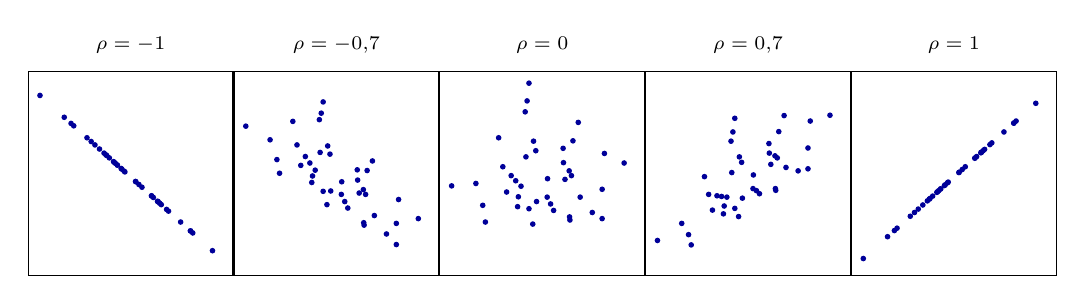
\begin{tikzpicture}
\begin{axis}[nuage, name=a, title={$\rho=-1$}]
  \addplot[point] coordinates {(-1.04,1.04) (0.22,-0.22) (-2.39,2.39) (1.64,-1.64) (0.71,-0.71) (-0.43,0.43) (-0.45,0.45) (0.30,-0.30) (-0.40,0.40) (-0.35,0.35) (0.81,-0.81) (0.56,-0.56) (-0.15,0.15) (-0.17,0.17) (0.13,-0.13) (-0.82,0.82) (-0.56,0.56) (0.60,-0.60) (-0.23,0.23) (-1.75,1.75) (-0.65,0.65) (0.73,-0.73) (-0.35,0.35) (-0.25,0.25) (0.72,-0.72) (2.16,-2.16) (-0.94,0.94) (1.58,-1.58) (-1.57,1.57) (0.14,-0.14) (-1.50,1.50) (1.58,-1.58) (0.95,-0.95) (1.32,-1.32) (-1.15,1.15) (0.77,-0.77) (-0.70,0.70) (-0.63,0.63) (0.55,-0.55) (1.00,-1.00)};
\end{axis}
\begin{axis}[nuage, name=b, at={([xshift=0.3cm]a.outer east)}, anchor=outer west, title={$\rho=-0{,}7$}]
  \addplot[point] coordinates {(-1.04,0.94) (0.22,-0.72) (-2.39,1.49) (1.64,-0.66) (0.71,-0.37) (-0.43,0.72) (-0.45,1.68) (0.30,-0.91) (-0.40,1.87) (-0.35,2.20) (0.81,0.19) (0.56,-0.09) (-0.15,-0.41) (-0.17,0.67) (0.13,-0.51) (-0.82,0.60) (-0.56,0.20) (0.60,-0.47) (-0.23,0.91) (-1.75,1.09) (-0.65,-0.16) (0.73,-1.41) (-0.35,-0.42) (-0.25,-0.81) (0.72,-1.34) (2.16,-1.22) (-0.94,0.34) (1.58,-1.36) (-1.57,0.51) (0.14,-0.14) (-1.50,0.11) (1.58,-1.98) (0.95,0.47) (1.32,-1.67) (-1.15,1.63) (0.77,-0.51) (-0.70,0.41) (-0.63,0.03) (0.55,0.21) (1.00,-1.13)};
\end{axis}
\begin{axis}[nuage, name=c, at={([xshift=0.3cm]b.outer east)}, anchor=outer west, title={$\rho=0$}]
  \addplot[point] coordinates {(-1.04,0.30) (0.22,-0.79) (-2.39,-0.26) (1.64,0.69) (0.71,0.18) (-0.43,0.59) (-0.45,1.91) (0.30,-0.98) (-0.40,2.23) (-0.35,2.75) (0.81,1.06) (0.56,0.42) (-0.15,-0.72) (-0.17,0.77) (0.13,-0.59) (-0.82,0.04) (-0.56,-0.27) (0.60,-0.07) (-0.23,1.05) (-1.75,-0.19) (-0.65,-0.87) (0.73,-1.26) (-0.35,-0.93) (-0.25,-1.38) (0.72,-1.17) (2.16,0.41) (-0.94,-0.44) (1.58,-0.36) (-1.57,-0.83) (0.14,-0.05) (-1.50,-1.32) (1.58,-1.22) (0.95,1.60) (1.32,-1.04) (-1.15,1.15) (0.77,0.04) (-0.70,-0.11) (-0.63,-0.58) (0.55,0.84) (1.00,-0.59)};
\end{axis}
\begin{axis}[nuage, name=d, at={([xshift=0.3cm]c.outer east)}, anchor=outer west, title={$\rho=0{,}7$}]
  \addplot[point] coordinates {(-1.04,-0.51) (0.22,-0.40) (-2.39,-1.86) (1.64,1.64) (0.71,0.62) (-0.43,0.13) (-0.45,1.05) (0.30,-0.49) (-0.40,1.32) (-0.35,1.72) (0.81,1.33) (0.56,0.70) (-0.15,-0.62) (-0.17,0.43) (0.13,-0.34) (-0.82,-0.55) (-0.56,-0.59) (0.60,0.37) (-0.23,0.59) (-1.75,-1.36) (-0.65,-1.08) (0.73,-0.39) (-0.35,-0.92) (-0.25,-1.16) (0.72,-0.34) (2.16,1.81) (-0.94,-0.97) (1.58,0.85) (-1.57,-1.69) (0.14,0.06) (-1.50,-1.99) (1.58,0.24) (0.95,1.80) (1.32,0.18) (-1.15,0.01) (0.77,0.56) (-0.70,-0.57) (-0.63,-0.85) (0.55,0.98) (1.00,0.28)};
\end{axis}
\begin{axis}[nuage, at={([xshift=0.3cm]d.outer east)}, anchor=outer west, title={$\rho=1$}]
  \addplot[point] coordinates {(-1.04,-1.04) (0.22,0.22) (-2.39,-2.39) (1.64,1.64) (0.71,0.71) (-0.43,-0.43) (-0.45,-0.45) (0.30,0.30) (-0.40,-0.40) (-0.35,-0.35) (0.81,0.81) (0.56,0.56) (-0.15,-0.15) (-0.17,-0.17) (0.13,0.13) (-0.82,-0.82) (-0.56,-0.56) (0.60,0.60) (-0.23,-0.23) (-1.75,-1.75) (-0.65,-0.65) (0.73,0.73) (-0.35,-0.35) (-0.25,-0.25) (0.72,0.72) (2.16,2.16) (-0.94,-0.94) (1.58,1.58) (-1.57,-1.57) (0.14,0.14) (-1.50,-1.50) (1.58,1.58) (0.95,0.95) (1.32,1.32) (-1.15,-1.15) (0.77,0.77) (-0.70,-0.70) (-0.63,-0.63) (0.55,0.55) (1.00,1.00)};
\end{axis}
\end{tikzpicture}
\end{center}

\end{frame}


\begin{frame}[t,label=excov]{Grappes de serveurs : covariance et corrélation}
Calculez la \alerter{covariance} et la \alerter{corrélation} entre le nombre de serveurs en panne dans
la grappe $\mathcal{X}$ et le nombre de serveurs en panne dans la grappe $\mathcal{Y}$.

\lienreponse{rep-ex2}
\end{frame}


\begin{frame}[t]{Grappes de serveurs : covariance et corrélation (suite)}

\lienreponse{rep-ex2}
\end{frame}


\begin{frame}[t]{Attention!}

Deux pièges à éviter au sujet de la corrélation :
\vspace{0.1in}
\begin{itemize}
\item $\rho(X,Y) = 0 \centernot\implies X \perp Y$ (contre-exemple à la diapo suivante);
\vspace{1.4in}
\item $\rho(X,Y)$ mesure la corrélation \textbf{linéaire}. Deux variables peuvent être reliées sans que
$\rho(X,Y)$ puisse le détecter.
\end{itemize}

\end{frame}


\begin{frame}[t,label=excontre]{Contre-exemple : corrélation nulle sans indépendance}

Soit $X$ et $Y$ de fonction de probabilité conjointe
\begin{center}
\begin{tabular}{cc|ccc}
$p(x,y)$ & & \multicolumn{3}{c}{$y$} \\
 & & 0 & 1 & 2 \\ \cline{1-5}
 & 0 & 0 & 1/4 & 0 \\
$x$ & 1 & 1/4 & 0 & 1/4 \\
 & 2 & 0 & 1/4 & 0 \\
\end{tabular}
\end{center}

Montrez que $\Cov(X,Y)=0$, mais que $X$ et $Y$ ne sont pas indépendantes.

\lienreponse{rep-ex2}
\end{frame}

% ============================================================================
\section{Combinaisons linéaires}

\begin{frame}[t]{Deux variables : espérance}

Soit deux v.a. $X$ et $Y$, et $W = a_1X + a_2Y$.

\medskip
$\alerter{E(W)}  =  E(a_1X + a_2Y)$\\
\phantom{$E(W)$}\ $=\ldots$

\end{frame}


\begin{frame}[t]{Deux variables : espérance (suite)}

\vfill
$$ \alerter{E(a_1X + a_2 Y) = a_1 E(X) + a_2 E(Y)}, \quad\text{que $X$ et $Y$ soient indépendantes ou non.}$$

\end{frame}


\begin{frame}[t]{Deux variables : variance}

\vspace{0.1in}
{\footnotesize
\begin{align*}
V(W) &=  E(W^2) - \{E(W)\}^2\\
 & = E\big[(a_1X + a_2Y )^2\big] - \{E(a_1X + a_2Y)\}^2\\
 & = E\big(a_1^2X^2 + 2a_1 a_2 X Y + a_2^2Y^2\big) - \{a_1E(X) + a_2 E(Y)\}^2  \\
 & = \ldots\\
 &= a_1^2 V(X) + 2 a_1 a_2 \Cov(X, Y) + a_2^2 V(Y)
\end{align*}
}

$$ \alerter{V(a_1X + a_2 Y) = a_1^2 V(X)  + a_2^2 V(Y) + 2 a_1 a_2 \Cov(X, Y) }$$

{\small Si $X\perp Y$, alors $\Cov(X,Y)=0$ et $V(a_1X+a_2Y)=a_1^2V(X)+a_2^2V(Y)$.}

\end{frame}


\begin{frame}[t]{Généralisation à plusieurs variables}
Soit $X_1,\ldots,X_n$ des variables aléatoires, $a_0,a_1,\ldots,a_n$ des constantes et
$Y=a_0+a_1X_1+\cdots+a_nX_n$. Alors
$$E(Y)=a_0+\sum_{i=1}^na_iE(X_i),$$
$$V(Y) =\sum_{i=1}^na_i^2V(X_i)+2\sum\limits_{j}\sum\limits_{i<j}a_ia_j\Cov(X_i,X_j)$$
{\small (le deuxième terme vaut deux fois la somme des covariances de toutes les paires).}

\vspace{0.1in}
Si $X_1,\ldots,X_n$ sont des v.a. \alerter{indépendantes}, alors $\Cov(X_i,X_j)=0$ et
$$V(Y)=\sum_{i=1}^na_i^2V(X_i).$$

\end{frame}


\begin{frame}[t,label=exdisque]{Exemple : espace disque d'un serveur de fichiers}

{\small
Chaque jour, deux applications écrivent des données sur un serveur de fichiers : $X_1$ et $X_2$
sont les volumes écrits (en Go), compressés à 60\,\% et à 50\,\% de leur taille. Une tâche de
nettoyage supprime $X_3$ fichiers temporaires de 1,6 Go chacun. La variation quotidienne de l'espace
occupé (en Go) est donc
$$Y=0{,}6X_1+0{,}5X_2-1{,}6X_3.$$

On sait que $E(X_1)=10$, $E(X_2)=20$, $E(X_3)=10$, $V(X_1)=4$, $V(X_2)=16$, $V(X_3)=1$,
$\Cov(X_1,X_2)=1{,}6$ et que $X_3$ est indépendante de $X_1$ et de $X_2$.

\vspace{0.1in}
Calculez l'espérance et la variance de $Y$, la variation quotidienne de l'espace occupé.
}
\lienreponse{rep-ex2}
\end{frame}


\begin{frame}[t]{Exemple : espace disque d'un serveur de fichiers (suite)}

\lienreponse{rep-ex2}
\end{frame}

% ============================================================================
\section{Compléments}

\begin{frame}[t,label=exautre]{Loi conjointe à partir des lois marginales?}
Soit $X$ et $Y$ deux v.a. de fonctions de probabilité respectives $p_X(x)=1/3$ pour $x=1,2$ et
$p_X(x)=1/6$ pour $x=3,4$, et $p_Y(y)=1/2$ pour $y=4,5$. Quelle est la fonction de probabilité
conjointe de $X$ et $Y$?

\lienreponse{rep-ex2}
\end{frame}

% ============================================================================
\section{Réponses des exemples}

\begin{frame}[t,label=rep-ex1]{Réponses des exemples (1/2)}
\footnotesize
\begin{itemize}\itemsep4pt
\item \retour{exgrappes}{Grappes de serveurs : lois marginales} : $p_X(0)=0{,}4$, $p_X(1)=0{,}35$,
$p_X(2)=0{,}25$~; $p_Y(0)=0{,}4$, $p_Y(1)=0{,}3$, $p_Y(2)=0{,}15$, $p_Y(3)=0{,}15$.
\item \textbf{Lois marginales (suite)} : $P(X=0)=p_X(0)=0{,}4$~; $E(X)=0\times0{,}4+1\times0{,}35+2\times0{,}25=0{,}85$ serveur.
\item \retour{excond}{Lois conditionnelles sachant $X=2$} : $p_{Y|2}(0)=0{,}4$, $p_{Y|2}(1)=0{,}2$,
$p_{Y|2}(2)=0{,}2$, $p_{Y|2}(3)=0{,}2$~; (suite) $P(Y=1|X=2)=0{,}2$.
\item \retour{exespcond}{Espérance conditionnelle} : $E[Y|2]=1{,}2$ serveur~;
$E[Y^2|2]=2{,}8$, d'où $V[Y|2]=2{,}8-1{,}2^2=1{,}36$.
\end{itemize}
\end{frame}


\begin{frame}[t,label=rep-ex2]{Réponses des exemples (2/2)}
\footnotesize
\begin{itemize}\itemsep4pt
\item \retour{exevenements}{Événements indépendants?} : oui, $P(E_1\cap E_2)=0{,}15=P(E_1)P(E_2)=0{,}25\times0{,}6$.
\item \retour{exindep}{Variables indépendantes?} : non, par exemple $p(0,3)=0\neq p_X(0)p_Y(3)=0{,}06$
(ou $p(0,0)=0{,}2\neq p_X(0)p_Y(0)=0{,}16$).
\item \retour{excov}{Covariance et corrélation} : $E(X)=0{,}85$, $E(Y)=1{,}05$, $E(XY)=1{,}1$~;
$\Cov(X,Y)=1{,}1-0{,}85\times1{,}05=0{,}2075$~; $V(X)=0{,}6275$, $V(Y)=1{,}1475$, d'où $\rho\approx 0{,}245$.
\item \retour{excontre}{Contre-exemple} : $E(X)=E(Y)=1$ et $E(XY)=1$, donc $\Cov(X,Y)=0$~; mais
$p(0,0)=0\neq p_X(0)p_Y(0)=1/16$.
\item \retour{exdisque}{Espace disque d'un serveur de fichiers} : $E(Y)=0$~Go~; $V(Y)=8{,}96$~Go$^2$.
\item \retour{exautre}{Loi conjointe à partir des lois marginales?} (compléments) : impossible sans
hypothèse supplémentaire~; si $X\perp Y$, $p(x,y)=1/6$ pour $x=1,2$ et $p(x,y)=1/12$ pour $x=3,4$ ($y=4,5$).
\end{itemize}
\end{frame}

% ============================================================================
\section{Réponses des quiz}

\begin{frame}[t,label=rep-quiz]{Réponses des quiz}
\footnotesize
\begin{itemize}\itemsep4pt
\item \retour{quizcov}{Quiz} ($\Cov(5,X)$) : $\Cov(5,X)=E(5X)-5E(X)=0$ (la covariance avec une constante est toujours nulle).
\item \textbf{Quiz} ($\Cov(X,3Y)=\Cov(Y,3X)$?) : vrai, car $\Cov(X,3Y)=3\Cov(X,Y)=\Cov(Y,3X)$.
\item \textbf{Quiz} (unités de la covariance) : $^\circ$C $\times$ secondes.
\end{itemize}
\end{frame}


\begin{frame}{Bibliographie}
 	Ce document est rédigé avec Beamer ainsi qu'une classe .cls fournie par Jérôme Soucy. Les diapositives sont adaptées des diapositives créées par Anne-Sophie Charest
 pour le cours STT-1000 ainsi que celles créées par Thierry Duchesne et Emmanuelle Reny-Nolin pour le cours STT-1900.
 	\printbibliography
 	\vfill
 	\footnotesize Pour signaler une erreur dans ce document, veuillez écrire à l'adresse :~\href{mailto:julien.miron@mat.ulaval.ca}{julien.miron@mat.ulaval.ca}.
 \end{frame}

\end{document}
